\documentclass{amsart}
\usepackage[T1]{fontenc}
\usepackage{lmodern}
\usepackage{amssymb}
\usepackage{graphicx}
\usepackage{booktabs}
\usepackage[hidelinks]{hyperref}

\newtheorem{theorem}{Theorem}[section]
\newtheorem{lemma}[theorem]{Lemma}
\newtheorem{proposition}[theorem]{Proposition}
\newtheorem{corollary}[theorem]{Corollary}
\theoremstyle{definition}
\newtheorem{definition}[theorem]{Definition}
\theoremstyle{remark}
\newtheorem{remark}[theorem]{Remark}

\numberwithin{equation}{section}

\newcommand{\N}{\mathbb{N}}
\newcommand{\gp}[1]{[#1]}
\newcommand{\repoURL}{https://github.com/creelie/ErdosProblem1}
\newcommand{\preprintURL}{https://github.com/creelie/ErdosProblem1/blob/main/preprintErdosStrausSieveConstant/ErdosStrausSieveConstant.pdf}

\makeatletter
\let\write@bibliographystyle\relax
\let\bibliography@latex\@gobble
\makeatother

\begin{document}

\title[The exact constant of the Erd\H{o}s--Straus sieve]{The exact constant of the two-parameter Type~II sieve for the Erd\H{o}s--Straus equation}

\author[D. Bhattacharjee]{Deep Bhattacharjee}
\address{Formerly, Electro-Gravitational Space Propulsion Laboratory (EGSPL),\newline Bhubaneswar, Odisha 751030, India; Formerly, University of Calcutta, Senate House,\newline 87/1 College Street, Kolkata 700073, West Bengal, India}
\email{itsdeep@live.com}
\email{d.bhattacharjee@erl-forschung.de}
\urladdr{https://orcid.org/0000-0003-0466-750X}
\thanks{Corresponding author: Deep Bhattacharjee.}

\author[U. Bhattacharya]{Ushashi Bhattacharya}
\address{Formerly, National Taiwan University, Taipei 106319, Taiwan}
\email{rai.bhattacharya.in@gmail.com}
\urladdr{https://orcid.org/0009-0002-2254-3914}

\subjclass[2020]{Primary 11D68; Secondary 11N36, 11N37, 11A25}
\keywords{Erd\H{o}s--Straus conjecture, Egyptian fractions, sieve methods, Euler totient function}

\begin{abstract}
We find the exact asymptotic size of the weighted count of search pairs that controls a recent sieve bound for the Erd\H{o}s--Straus equation, settling the first open question left by that work. The leading constant is three times the one previously proved, and the exponents of the resulting bounds for the exceptional primes improve accordingly.
\end{abstract}

\maketitle

\setcounter{tocdepth}{1}
\tableofcontents

\section{Introduction}
\enlargethispage{3pt}

The Erd\H{o}s--Straus conjecture, posed in 1948, asserts that for every integer $n\ge2$ the equation
\begin{equation}\label{eq:es}
\frac4n=\frac1x+\frac1y+\frac1z
\end{equation}
has a solution in positive integers $x,y,z$ \cite[\S D11]{Guy}. A solution for $n$ gives one for every multiple of $n$, so it is enough to treat primes, and polynomial identities settle every prime outside the six residue classes $1,121,169,289,361,529$ modulo $840$ \cite{Mor}. These are the squares of the classes coprime to $840$, and Mordell's barrier says that no identity of this kind can settle a square class, so the remaining primes cannot be reached by congruences alone.\footnote{More precisely, a polynomial identity solving \eqref{eq:es} for all $n$ in a residue class $r$ modulo $q$ exists only if $r$ is not a square modulo $q$; see \cite[Section~2]{ET} for a proof of this principle and for the families of identities behind it. The same obstruction is visible in practice: a search over the Type~II identities of Section~\ref{sec:typeII} with small parameters leaves, among the integers below $10^8$ in the six classes, exactly the perfect squares.} The conjecture has been verified for all $n\le10^{17}$ by Salez \cite{Sal} and for all $n\le10^{18}$ by Mihnea and Dumitru \cite{MD}, and Vaughan showed that the number of exceptions up to $N$ is at most $N\exp(-c(\log N)^{2/3})$ \cite{Vau}. Elsholtz and Tao \cite{ET} divided the solutions of \eqref{eq:es} for a prime $n$ into Type~I, in which $n$ divides exactly one of $x,y,z$, and Type~II, in which it divides two of them, and determined the average number of solutions of each type. The conjecture remains open.

Dahan \cite{Dah} recently asked how deep a search has to go before it finds a Type~II solution. He showed that a prime $n$ has a Type~II solution if and only if there are positive integers $u$ and $a$ such that
\begin{equation}\label{eq:criterion}
an+u \text{ has a divisor } s\equiv-1\pmod{4ua},
\end{equation}
and that one may take $u$ and $a$ coprime (Section~\ref{sec:typeII}). Let $E_2(N;J)$ be the set of primes $n\le N$ with $n\equiv1\pmod{24}$ for which \eqref{eq:criterion} has no solution with coprime $u,a\le J$. Dahan bounds $|E_2(N;J)|$ by a sieve whose size is governed by the sum
\begin{equation}\label{eq:W}
W(J)=\sum_{\substack{u,a\le J\\ \gcd(u,a)=1}}\frac1{\varphi(4ua)},
\end{equation}
which counts the residue classes $-1$ modulo $4ua$ with the weight that each class receives among the primes.\footnote{By the prime number theorem in arithmetic progressions, the primes $p\le x$ with $p\equiv-1\pmod{4ua}$ number about $\pi(x)/\varphi(4ua)$, so $W(J)$ is the expected number of pairs $(u,a)$ for which a prime divisor of the right size lies in the right class. The use of the large sieve in this setting is in the spirit of \cite{BB26}, where it controls Liouville correlations uniformly in the coefficients.} Using $\varphi(m)\le m$ he proved $W(J)\ge(\kappa_1+o(1))(\log J)^2$ with $\kappa_1=3/(2\pi^2)=0.15198\ldots$ \cite[Lemma~4.22]{Dah}. He observed numerically that $W(J)/(\log J)^2$ seems to tend to a limit near $0.46$, and the first of the questions with which he closes his paper is to prove $W(J)\ge(0.45+o(1))(\log J)^2$ \cite[Section~7]{Dah}. We determine $W(J)$ up to an error that tends to zero.

\begin{theorem}\label{thm:main}
Let
\[
\kappa=\frac9{2\pi^2}=0.4559453263\ldots,\qquad T=\frac{\log2}3+\sum_{p>2}\frac{\log p}{(p-1)(p^2+1)},
\]
\[
M=-\frac49(\log2)^2-\sum_{p>2}(\log p)^2\Bigl(\frac{p+1}{(p-1)(p^2+1)}+\frac1{(p-1)^2(p^2+1)^2}\Bigr),
\]
the sums running over odd primes, and let $\gamma$ be Euler's constant. Then, for $J\ge2$,
\[
W(J)=\kappa\bigl((\log J+\gamma+T)^2+M\bigr)+O\bigl(J^{-1/2}\log J\bigr).
\]
Numerically $T=0.3131549610\ldots$ and $M=-1.0429405079\ldots$, so that
\[
W(J)=\kappa(\log J)^2+0.8119206513\ldots\log J-0.1140687011\ldots+O\bigl(J^{-1/2}\log J\bigr).
\]
\end{theorem}

In particular $W(J)\sim\kappa(\log J)^2$ with $\kappa=3\kappa_1$, which answers Dahan's question; the limit near $0.46$ that he extrapolated from four values of $W(J)$ is $\kappa=0.45594\ldots$. Figure~\ref{fig:ratio} compares the formula with $W(J)$ computed exactly.

\begin{figure}[ht]
\centering
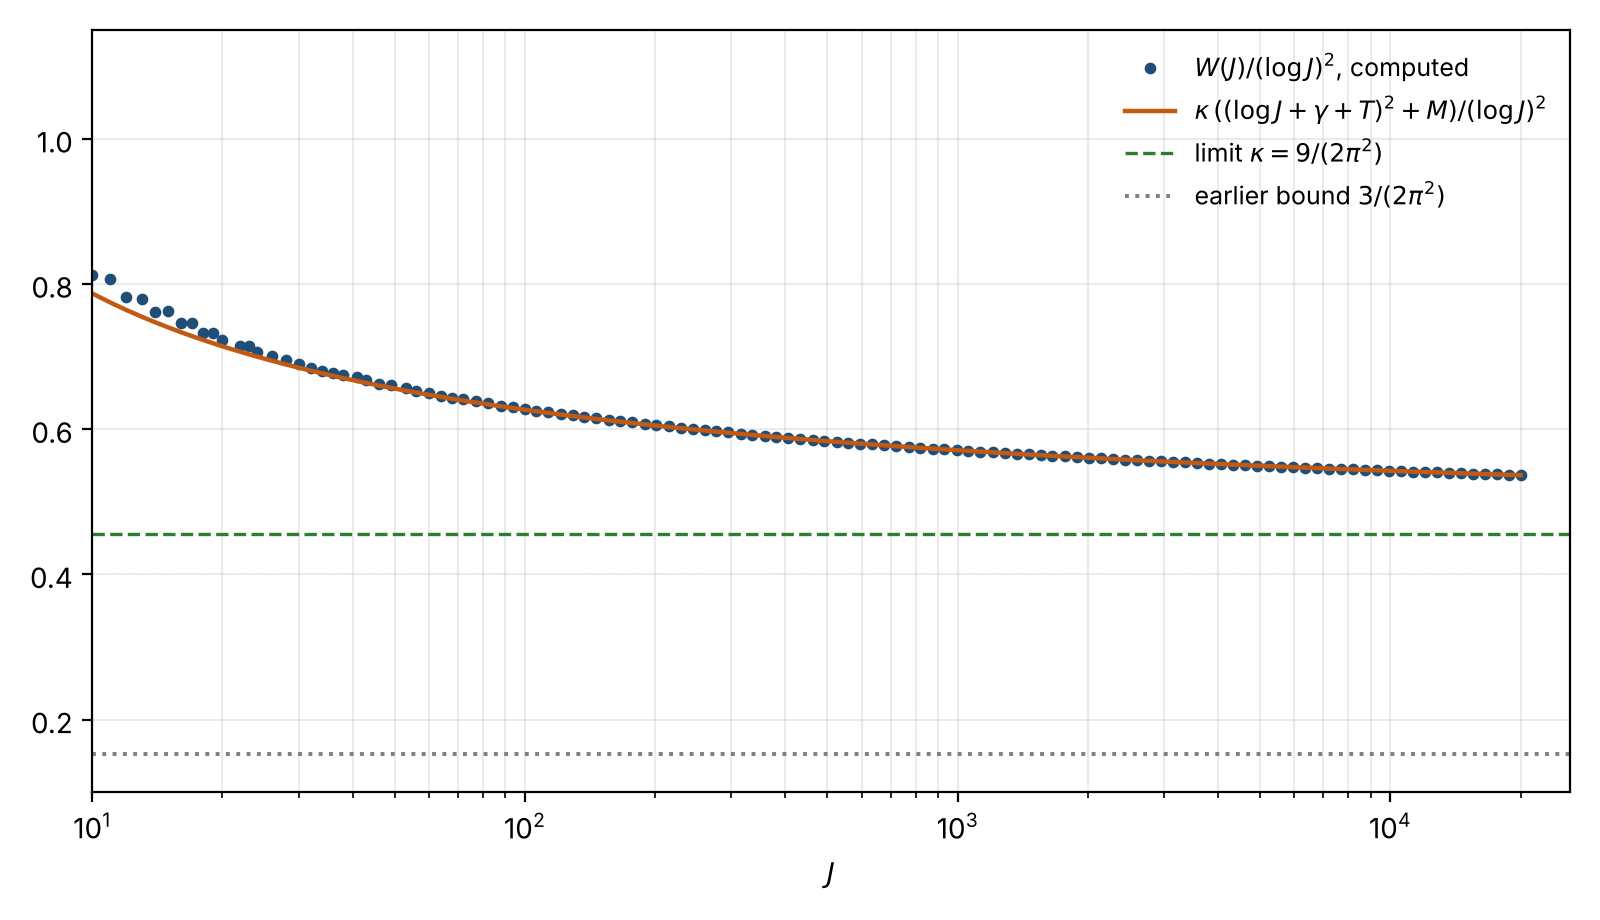
\includegraphics[width=0.95\textwidth]{figures/fig_ratio.png}
\caption{The ratio $W(J)/(\log J)^2$ computed from \eqref{eq:W} for $10\le J\le 2\cdot10^4$ (dots), the three-term formula of Theorem~\ref{thm:main} divided by $(\log J)^2$ (solid line), its limit $\kappa=9/(2\pi^2)$ (dashed) and the constant $3/(2\pi^2)$ proved in \cite{Dah} (dotted). The ratio approaches $\kappa$ slowly, as $1+2(\gamma+T)/\log J$, which is why it is still above $0.53$ at $J=2\cdot10^4$.}
\label{fig:ratio}
\end{figure}

Dahan's sieve uses $W(J)$ only through a lower bound, and he notes that every constant of \cite[Section~4.3]{Dah} improves as soon as a sharper lower bound is proved \cite[p.~28]{Dah}. Substituting Theorem~\ref{thm:main} into his arguments gives the following bounds; they rest on the arguments of \cite{Dah}, which we use as stated and have not verified beyond the step in which $W(J)$ enters.

\begin{corollary}\label{cor:depth}
Let $\kappa=9/(2\pi^2)$. In the setting of \cite[Section~4.3]{Dah}:
\begin{enumerate}
\item for fixed $\lambda\ge1$ and $J=(\log N)^\lambda$,
\[
|E_2(N;J)|\ll N\exp\bigl(-(\kappa\lambda^2+o(1))(\log\log N)^3\bigr),
\]
against $\kappa_1\lambda^2$ in \cite[Theorem~4.17]{Dah};
\item with $J=(\log N)^\lambda$ and $z=\exp(\sqrt{\log N})$ the exponent is
\[
(\kappa/2+o(1))\lambda^2(\log\log N)^3,
\]
against $\kappa_1/2$ in \cite[Corollary~4.29]{Dah};
\item with the choices
\[
\log z=\Bigl(\frac{25e\log N}{\kappa}\Bigr)^{1/3}=5.302\ldots(\log N)^{1/3},
\]
\[
\log J=\frac{\log z}{5\sqrt e}=0.643\ldots(\log N)^{1/3},
\]
\[
|E_2(N;J)|\ll N\exp\bigl(-0.0943\,(\log N)^{2/3}\bigr),
\]
against $0.065$ in \cite[Corollary~4.31]{Dah}.
\end{enumerate}
\end{corollary}

The constant in (3) is $\frac12(\kappa/(25e))^{1/3}=0.09430385\ldots$, which is $3^{1/3}$ times Dahan's $0.06538\ldots$. Corollary~\ref{cor:depth} concerns the search depth only: it bounds the number of primes for which a Type~II solution, if one exists, is not found among small parameters, and it says nothing about the primes for which no solution exists. It does not prove the Erd\H{o}s--Straus conjecture.

The proof of Theorem~\ref{thm:main} rests on one observation: although $1/\varphi(4ua)$ is not a multiplicative function of the pair $(u,a)$, the quantity $ua/\varphi(4ua)$ is, after the factor $\frac12$ coming from the prime $2$ is removed. Its Dirichlet inverse with respect to both variables is supported on squarefree pairs and decays fast enough to make a two-variable version of the familiar argument for $\sum_{n\le x}1/\varphi(n)$ \cite{Mon} work with a power saving. Section~\ref{sec:typeII} recalls the criterion \eqref{eq:criterion} with the identity behind it, Section~\ref{sec:mult} contains the multiplicative structure, Section~\ref{sec:proof} the proof, Section~\ref{sec:constants} the constants and the numerical comparison, and Section~\ref{sec:verification} the formal and numerical checks.

\section{The Type II identity}\label{sec:typeII}

The criterion \eqref{eq:criterion} comes from an identity that we record because it gives the solution explicitly.

\begin{lemma}\label{lem:identity}
Let $n,u,a$ be positive integers and let $s$ be a divisor of $an+u$ with $s\equiv-1\pmod{4ua}$. Write $s+1=4ua\alpha$ and $an+u=sv$. Then
\begin{equation}\label{eq:identity}
\frac4n=\frac1{\alpha uv}+\frac1{a\alpha nu}+\frac1{a\alpha nv}.
\end{equation}
\end{lemma}

\begin{proof}
The right-hand side equals $(an+u+v)/(a\alpha nuv)$. Since $an+u=sv=(4a\alpha u-1)v$, the numerator is $4a\alpha uv$, and the fraction is $4/n$.
\end{proof}

For the prime $n=409$ one may take $u=1$, $a=2$ and $s=7$, which divides $819=7\cdot117$; then $\alpha=1$, $v=117$, and \eqref{eq:identity} reads $4/409=1/117+1/818+1/95706$. When $n$ is prime and $n\nmid uv$, two of the three denominators in \eqref{eq:identity} are divisible by $n$ and the third is not, so the solution is of Type~II. Conversely every Type~II solution arises in this way \cite[Theorem~3.9]{Dah}, \cite[Section~2]{ET}. If $s$ is a witness for $(u,a)$ and $d=\gcd(u,a)$, then $s$ is coprime to $d$, because $d\mid s+1$, and so $s$ divides $(a/d)n+u/d$ and is $\equiv-1$ modulo $4(u/d)(a/d)$; hence the coprime pairs suffice \cite[Lemma~3.10]{Dah}, which is why the sum \eqref{eq:W} is restricted to them.\footnote{Figure~\ref{fig:terms} shows the terms of \eqref{eq:W}. A single prime $p\equiv-1\pmod{4ua}$ dividing $an+u$ gives a witness, and the density of such primes is $1/\varphi(4ua)$; this is the source of the weight in \eqref{eq:W}.}

\begin{figure}[ht]
\centering
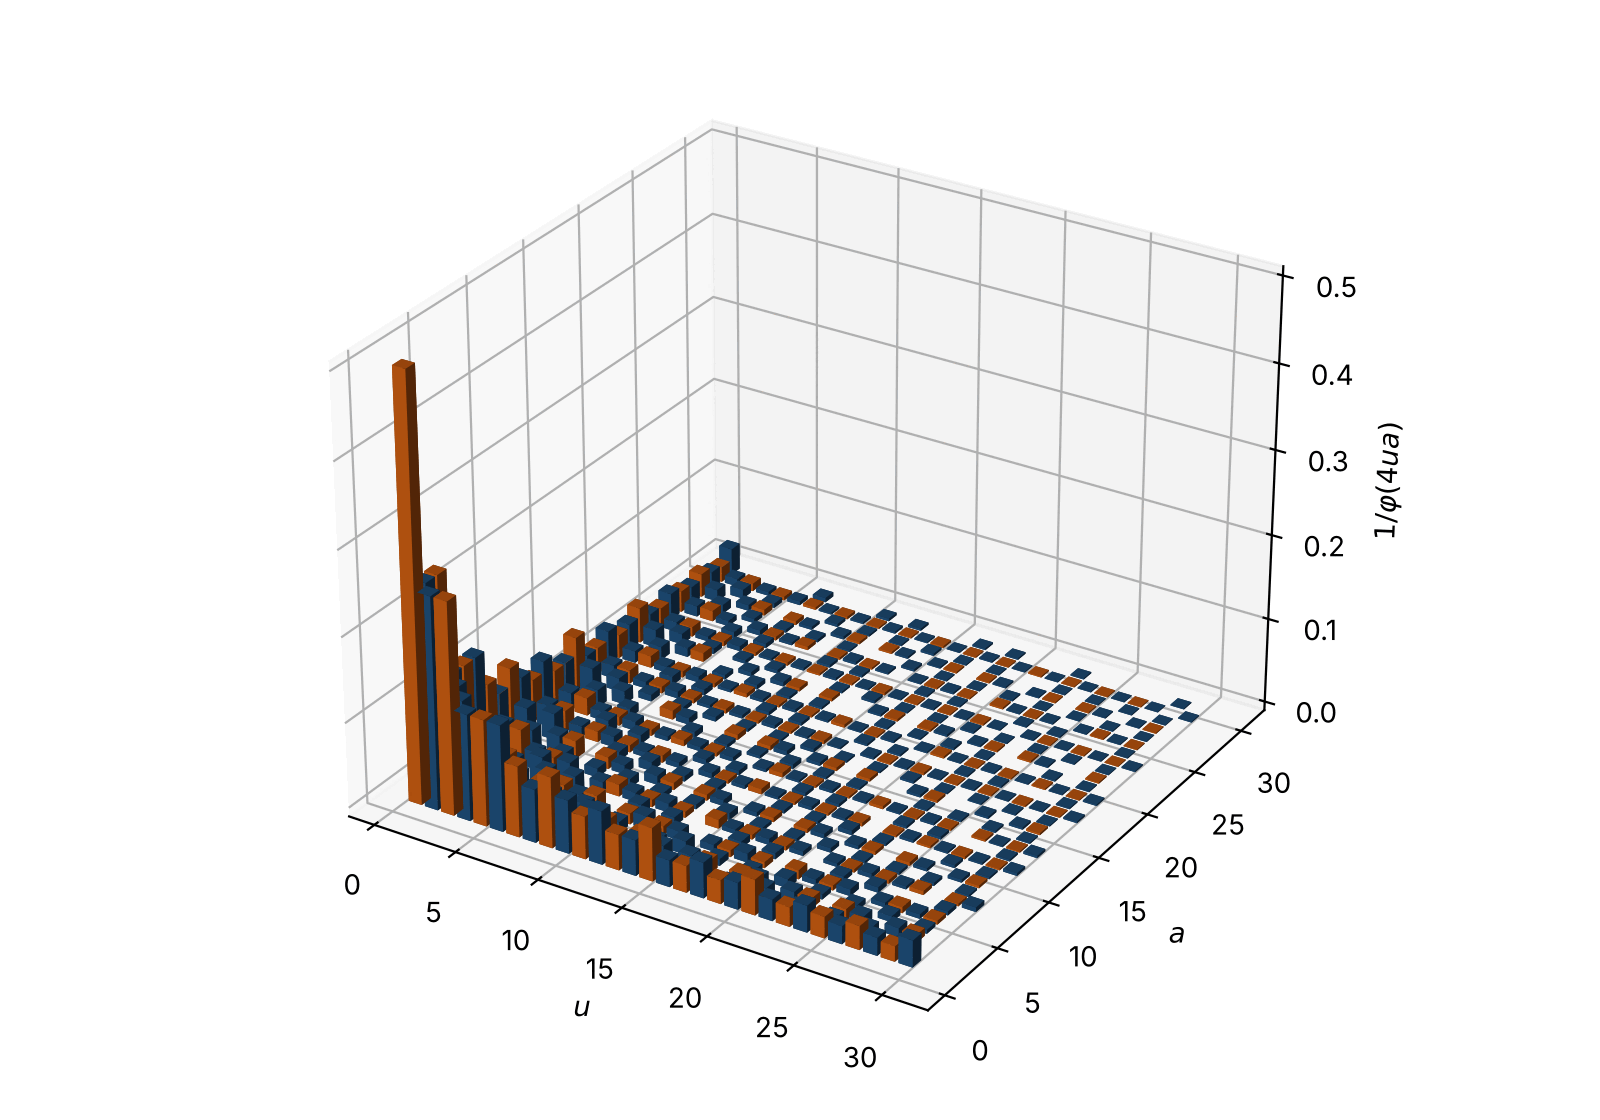
\includegraphics[width=0.78\textwidth]{figures/fig_terms.png}
\caption{The terms $1/\varphi(4ua)$ of the sum \eqref{eq:W} for coprime $u,a\le30$; orange bars are the pairs with $ua$ odd and blue bars those with $ua$ even. Missing bars are the pairs with $\gcd(u,a)>1$. By Lemma~\ref{lem:factor} an even product $ua$ halves the weight, which is the source of the factor $3/4$ at the prime $2$ in \eqref{eq:Z00}.}
\label{fig:terms}
\end{figure}

\section{A multiplicative function of two variables}\label{sec:mult}

For a positive integer $m$ write $m'$ for its largest odd divisor, and put $g(m)=m/\varphi(m)$.

\begin{lemma}\label{lem:factor}
For coprime positive integers $u$ and $a$,
\[
\frac{ua}{\varphi(4ua)}=\frac12\,g(u')\,g(a').
\]
\end{lemma}

\begin{proof}
Write $u=2^\beta u'$ and $a=2^\delta a'$; since $\gcd(u,a)=1$, the integers $2^{2+\beta+\delta}$, $u'$, $a'$ are pairwise coprime, so $\varphi(4ua)=2^{1+\beta+\delta}\varphi(u')\varphi(a')$. Dividing $ua=2^{\beta+\delta}u'a'$ by this gives the claim.
\end{proof}

Consequently
\begin{equation}\label{eq:Wh}
W(J)=\frac12\sum_{u,a\le J}\frac{h(u,a)}{ua},\qquad h(u,a)=[\gcd(u,a)=1]\,g(u')\,g(a'),
\end{equation}
where $[\,\cdot\,]$ is $1$ when the condition holds and $0$ otherwise. The function $h$ is multiplicative in the pair: $h(u_1u_2,a_1a_2)=h(u_1,a_1)h(u_2,a_2)$ whenever $\gcd(u_1a_1,u_2a_2)=1$. It is therefore determined by its values $h(p^i,p^j)$, which are
$h(1,1)=1$; $h(p^i,p^j)=0$ when $i,j\ge1$; and, when exactly one of $i,j$ is positive, $h(p^i,p^j)=p/(p-1)$ for odd $p$ and $h(p^i,p^j)=1$ for $p=2$.
Define $k$ by M\"obius inversion in both variables,
\[
k(d,e)=\sum_{d_1d_2=d}\ \sum_{e_1e_2=e}\mu(d_2)\mu(e_2)\,h(d_1,e_1),
\]
so that
\[
h(u,a)=\sum_{d\mid u}\sum_{e\mid a}k(d,e).
\]
The function $k$ is again multiplicative in the pair, and $k(p^i,p^j)=h(p^i,p^j)-h(p^{i-1},p^j)-h(p^i,p^{j-1})+h(p^{i-1},p^{j-1})$, with $h$ set to $0$ at negative exponents.

\begin{lemma}\label{lem:k}
For an odd prime $p$,
\[
k(p,1)=k(1,p)=\frac1{p-1},\qquad k(p,p)=-\frac{p+1}{p-1},
\]
and $k(2,2)=-1$. At every prime, $k(p^i,p^j)=0$ for all other pairs $(i,j)\ne(0,0)$.
\end{lemma}

\begin{proof}
For odd $p$, $k(p,1)=p/(p-1)-1=1/(p-1)$ and $k(p,p)=0-2p/(p-1)+1=-(p+1)/(p-1)$. If $i\ge2$ and $j=0$, the two values $h(p^i,1)$ and $h(p^{i-1},1)$ are both $p/(p-1)$, and the other two vanish. If $i\ge2$ and $j\ge1$, then $h(p^i,p^j)=h(p^{i-1},p^j)=0$ and $h(p^i,p^{j-1})=h(p^{i-1},p^{j-1})$, both being $0$ when $j\ge2$ and $p/(p-1)$ when $j=1$. The cases with $i$ and $j$ exchanged are symmetric. At $p=2$ the same computation with $p/(p-1)$ replaced by $1$ gives $k(2,1)=k(1,2)=0$, $k(2,2)=0-1-1+1=-1$, and $0$ elsewhere.
\end{proof}

Thus $k(d,e)\ne0$ only when $d=q_1q_3$ and $e=q_2q_3$ with $q_1,q_2,q_3$ squarefree and pairwise coprime and $q_1q_2$ odd. For real $\sigma,\tau$ consider
\[
Z(\sigma,\tau)=\sum_{d,e\ge1}\frac{k(d,e)}{d^{1+\sigma}e^{1+\tau}}=\prod_pE_p(\sigma,\tau),
\]
where, for odd $p$,
\[
E_p(\sigma,\tau)=1+\frac1{(p-1)p^{1+\sigma}}+\frac1{(p-1)p^{1+\tau}}-\frac{p+1}{(p-1)p^{2+\sigma+\tau}},
\]
and $E_2(\sigma,\tau)=1-2^{-2-\sigma-\tau}$.
The series converges absolutely when $\sigma>-1$, $\tau>-1$ and $\sigma+\tau>-1$, because then the same product with every term replaced by its absolute value converges: its local factor is $1+O(p^{-2-\sigma}+p^{-2-\tau}+p^{-2-\sigma-\tau})$ and each exponent exceeds $1$. In this open region $Z$ is a convergent Euler product of nonvanishing factors, and the derivatives below may be taken term by term. We use the region at the points $(0,0)$ and $(-\tfrac12,0)$, $(0,-\tfrac12)$; in particular the constant
\[
A=\sum_{d,e}\frac{|k(d,e)|\,(1+\log d)^2(1+\log e)^2}{d^{1/2}e}
\]
and its mirror image are finite.

\begin{lemma}\label{lem:values}
\begin{align}
Z(0,0)&=\frac34\prod_{p>2}\Bigl(1+\frac1{p^2}\Bigr)=\frac9{\pi^2},\label{eq:Z00}\\
\frac{\partial}{\partial\sigma}\log Z(0,0)&=\frac{\partial}{\partial\tau}\log Z(0,0)=T,\label{eq:T}\\
\frac{\partial^2}{\partial\sigma\,\partial\tau}\log Z(0,0)&=M.\label{eq:M}
\end{align}
\end{lemma}

\begin{proof}
For odd $p$,
\[
E_p(0,0)=1+\frac2{p(p-1)}-\frac{p+1}{(p-1)p^2}=1+\frac{2p-p-1}{(p-1)p^2}=1+\frac1{p^2},
\]
and $E_2(0,0)=3/4$. Since $\prod_p(1+p^{-2})=\zeta(2)/\zeta(4)=15/\pi^2$ and the factor at $p=2$ is $5/4$, we obtain $Z(0,0)=\frac34\cdot\frac45\cdot\frac{15}{\pi^2}=\frac9{\pi^2}$. For the derivatives, write $\ell=\log p$. At odd $p$,
\[
\partial_\sigma E_p(0,0)=-\frac{\ell}{(p-1)p}+\frac{(p+1)\ell}{(p-1)p^2}=\frac{\ell}{(p-1)p^2},\qquad \partial_\sigma\partial_\tau E_p(0,0)=-\frac{(p+1)\ell^2}{(p-1)p^2},
\]
and dividing by $E_p(0,0)=(p^2+1)/p^2$ gives $\partial_\sigma\log E_p=\ell/((p-1)(p^2+1))$ and
\[
\partial_\sigma\partial_\tau\log E_p=\frac{\partial_\sigma\partial_\tau E_p}{E_p}-\frac{\partial_\sigma E_p\,\partial_\tau E_p}{E_p^2}=-\ell^2\Bigl(\frac{p+1}{(p-1)(p^2+1)}+\frac1{(p-1)^2(p^2+1)^2}\Bigr).
\]
At $p=2$, with $w=2^{-2-\sigma-\tau}$ we have $\log E_2=\log(1-w)$, $\partial_\sigma\log E_2=w\log2/(1-w)$ and $\partial_\sigma\partial_\tau\log E_2=-w(\log2)^2/(1-w)^2$; at $w=1/4$ these are $(\log2)/3$ and $-\frac49(\log2)^2$. Summing over $p$ gives \eqref{eq:T} and \eqref{eq:M}; the symmetry $E_p(\sigma,\tau)=E_p(\tau,\sigma)$ gives the equality of the two first derivatives.
\end{proof}

Figure~\ref{fig:region} shows the surface $\log Z$ near the point $(0,0)$; the theorem reads off its height, its two slopes and its mixed curvature there.

\begin{figure}[ht]
\centering
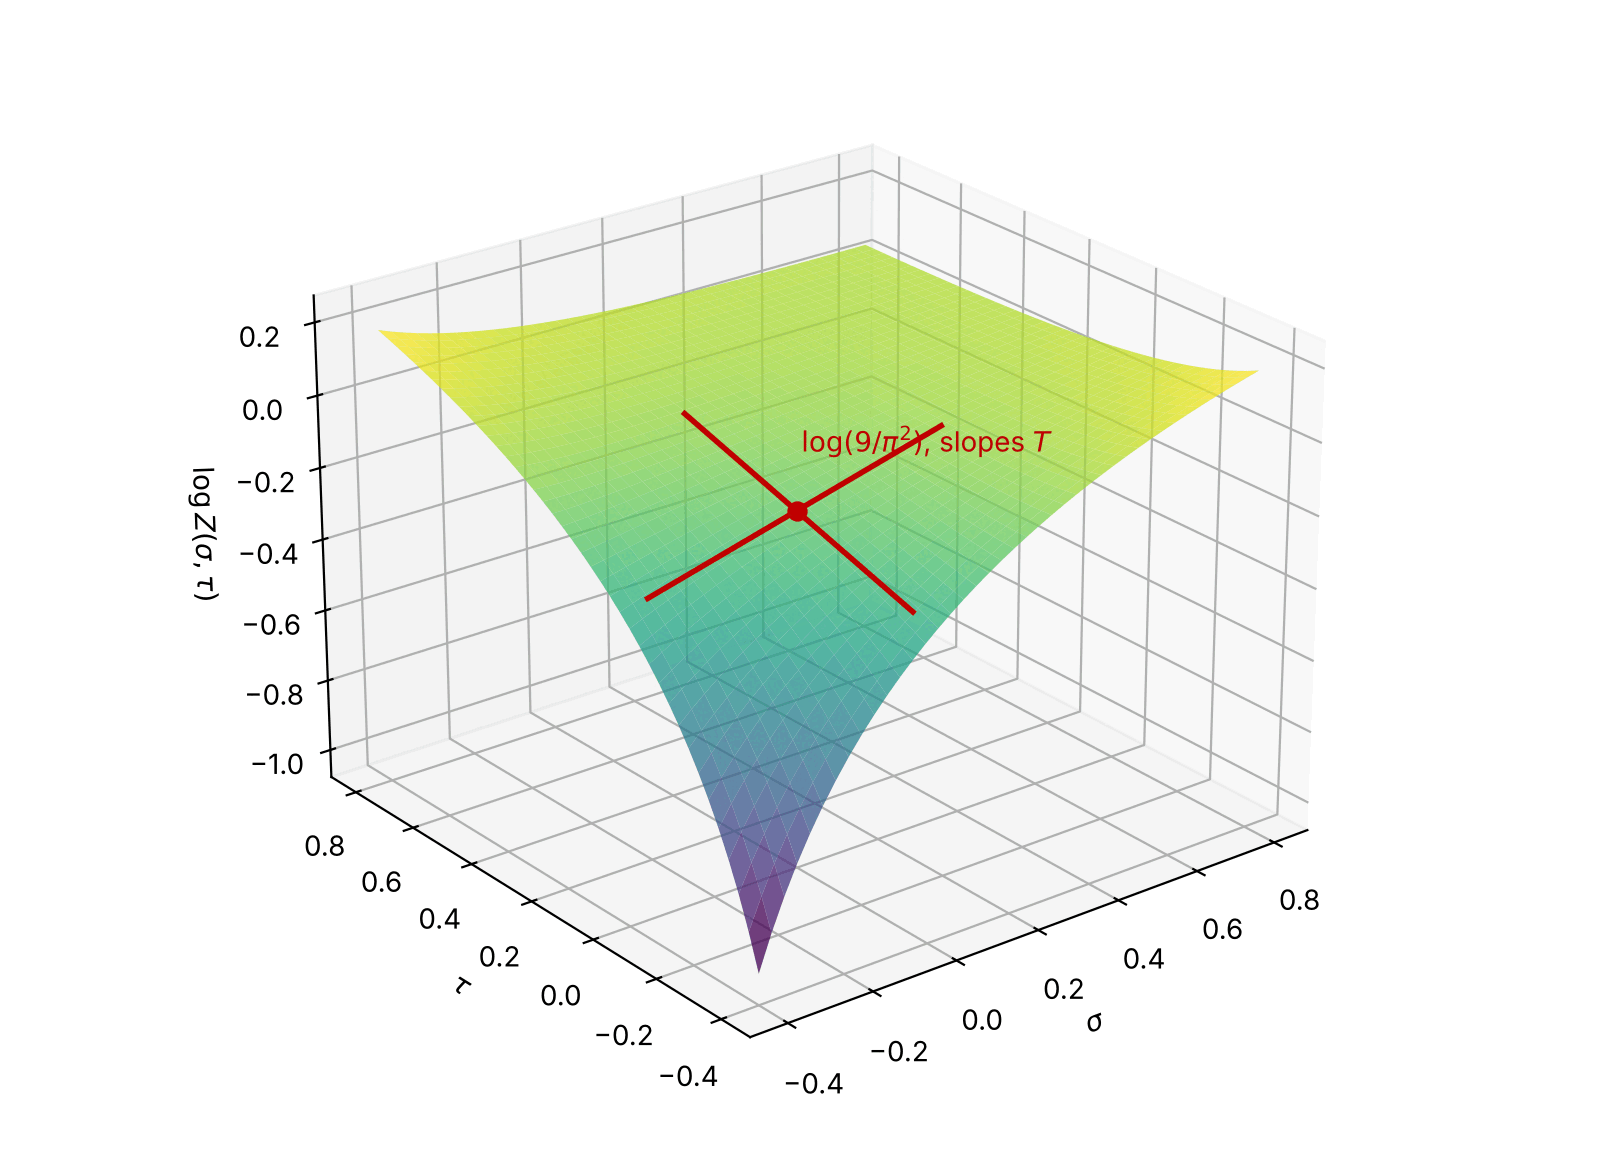
\includegraphics[width=0.8\textwidth]{figures/fig_region.png}
\caption{The surface $(\sigma,\tau)\mapsto\log Z(\sigma,\tau)$ over $-0.4\le\sigma,\tau\le0.8$, computed from the Euler product over the primes below $2\cdot10^5$. The marked point is $(0,0,\log(9/\pi^2))$, which gives the leading constant $\kappa=Z(0,0)/2$; the two lines through it have slope $T$ in the $\sigma$ and $\tau$ directions, and the mixed second derivative there is $M$. The surface drops steeply towards the corner $\sigma=\tau=-\frac12$, where the line $\sigma+\tau=-1$ bounds the region of absolute convergence.}
\label{fig:region}
\end{figure}

\section{Proof of Theorem \ref{thm:main}}\label{sec:proof}

Let $H(x)=\sum_{m\le x}1/m$ for $x\ge1$. By \eqref{eq:Wh} and the inversion formula,
\[
W(J)=\frac12\sum_{u,a\le J}\frac1{ua}\sum_{d\mid u,\ e\mid a}k(d,e)=\frac12\sum_{d,e\le J}\frac{k(d,e)}{de}\,H\Bigl(\frac Jd\Bigr)H\Bigl(\frac Je\Bigr),
\]
on writing $u=dm$, $a=en$. We use $H(x)=\log x+\gamma+R(x)$ with $|R(x)|\le 2/x$ for $x\ge1$ (Appendix~\ref{app:harmonic}).\footnote{The constant $\gamma$ enters only through this expansion, and it is the reason why Euler's constant appears beside the arithmetic constant $T$ in Theorem~\ref{thm:main}: each of the two harmonic sums contributes one $\gamma$, and the cross term $2\gamma T$ in $(\log J+\gamma+T)^2$ couples the archimedean part of the problem with the primes.} Put $L=\log J+\gamma$. Then $H(J/d)=L-\log d+R(J/d)$, and
\[
H\Bigl(\frac Jd\Bigr)H\Bigl(\frac Je\Bigr)=(L-\log d)(L-\log e)+R\Bigl(\frac Jd\Bigr)H\Bigl(\frac Je\Bigr)+R\Bigl(\frac Je\Bigr)(L-\log d).
\]

\emph{The remainder terms.} For $d,e\le J$ we have $0\le H(J/e)\le1+\log J$, $|L-\log d|\le1+\log J$ and $|R(J/d)|\le 2d/J\le2(d/J)^{1/2}$. Hence the two remainder terms, after multiplication by $\frac12|k(d,e)|/(de)$ and summation, contribute at most
\[
\frac{1+\log J}{J^{1/2}}\sum_{d,e}\frac{|k(d,e)|}{d^{1/2}e}+\frac{1+\log J}{J^{1/2}}\sum_{d,e}\frac{|k(d,e)|}{de^{1/2}}\le\frac{2A(1+\log J)}{J^{1/2}}.
\]

\emph{Completing the main term.} It remains to replace $\sum_{d,e\le J}$ by $\sum_{d,e\ge1}$ in
\[
\frac12\sum_{d,e}\frac{k(d,e)}{de}(L-\log d)(L-\log e).
\]
The pairs with $d>J$ satisfy $\log J<\log d$, so $|L-\log d|\le1+2\log d$ and $|L-\log e|\le 1+\log d+\log e$, and $1/d\le J^{-1/2}d^{-1/2}$; their contribution is therefore at most
\[
\frac1{J^{1/2}}\sum_{d,e}\frac{|k(d,e)|(1+2\log d)(1+\log d+\log e)}{d^{1/2}e}\le\frac{2A}{J^{1/2}}.
\]
The pairs with $e>J$ are treated in the same way, and the pairs with both $d,e>J$ are counted twice, which only helps the bound. So
\[
W(J)=\frac12\bigl(S_0L^2-2S_1L+S_{11}\bigr)+O\bigl(J^{-1/2}\log J\bigr),
\]
with
\[
S_0=\sum_{d,e}\frac{k(d,e)}{de},\qquad S_1=\sum_{d,e}\frac{k(d,e)\log d}{de}=\sum_{d,e}\frac{k(d,e)\log e}{de},
\]
\[
S_{11}=\sum_{d,e}\frac{k(d,e)\log d\log e}{de}.
\]
In terms of $Z$ these are $S_0=Z$, $S_1=-\partial_\sigma Z$ and $S_{11}=\partial_\sigma\partial_\tau Z$, all at $(0,0)$. By Lemma~\ref{lem:values}, $\partial_\sigma Z/Z=T$ and
\[
\frac{\partial_\sigma\partial_\tau Z}{Z}=\partial_\sigma\partial_\tau\log Z+\frac{\partial_\sigma Z}{Z}\cdot\frac{\partial_\tau Z}{Z}=M+T^2.
\]
Therefore
\[
\frac12\bigl(S_0L^2-2S_1L+S_{11}\bigr)=\frac{Z(0,0)}2\bigl(L^2+2TL+T^2+M\bigr)=\frac9{2\pi^2}\bigl((L+T)^2+M\bigr),
\]
which is Theorem~\ref{thm:main}. Expanding the square gives the second form, with the coefficient of $\log J$ equal to $2\kappa(\gamma+T)$ and the constant equal to $\kappa((\gamma+T)^2+M)$. \qed

\begin{remark}
The same argument applies to the one-parameter sum $\sum_{u\le J}1/\varphi(4u)$ of \cite[Lemma~4.21]{Dah}, where $4u/\varphi(4u)=2g(u')$ and one recovers the constant $\kappa_0=\zeta(2)\zeta(3)/(3\zeta(6))$ of that lemma. The two-variable case differs only in the diagonal value $k(p,p)$, which comes from the coprimality condition and produces the factor $1+p^{-2}$ in place of $1+1/(p(p-1))$.\footnote{The Euler factors $1+p^{-2}$ and the quotient $\zeta(2)/\zeta(4)$ that they produce are typical of sums over coprime pairs; a different instance, where the same quotient appears through Ramanujan's function, is studied in \cite{BBS23}. The two-variable inversion used here is the Dirichlet-series counterpart of the approximation arguments of \cite{BNFS26}, where a single-variable M\"obius sum has to be controlled with an explicit error.}
\end{remark}

\section{The constants}\label{sec:constants}

The series for $T$ converges like $\sum_p(\log p)p^{-3}$, and summing over the primes below $10^7$ determines it to twelve digits. The series for $M$ converges more slowly, like $\sum_p(\log p)^2p^{-2}$: by the prime number theorem the primes above $P$ contribute $(\log P+1)/P$ up to a factor $1+o(1)$, which is $1.7\cdot10^{-6}$ at $P=10^7$.\footnote{Summing over the primes up to $P=10^7$, $10^8$ and $4\cdot10^8$ gives $-1.0429387961$, $-1.0429403137$ and $-1.0429404559$; subtracting $(\log P+1)/P$ from each gives $-1.04294050791$, $-1.04294050795$ and $-1.04294050794$. The agreement of the corrected values to eleven digits, while the uncorrected ones move in the sixth, is the evidence for the digits of $M$ stated in the text.} Summing up to $4\cdot10^8$ and adding this correction gives
\[
T=0.3131549610\ldots,\qquad M=-1.0429405079\ldots,\qquad \gamma+T=0.8903706259\ldots,
\]
and hence $2\kappa(\gamma+T)=0.8119206513\ldots$ and $\kappa((\gamma+T)^2+M)=-0.1140687011\ldots$. Table~\ref{tab:W} compares the formula with $W(J)$ computed directly from \eqref{eq:W}. The first four values of the ratio $W(J)/(\log J)^2$ are those reported in \cite[Section~6, item~(8)]{Dah}.

\begin{table}[ht]
\centering
\caption{The sum $W(J)$, the formula $\kappa((\log J+\gamma+T)^2+M)$ of Theorem~\ref{thm:main}, their difference, and the ratio $W(J)/(\log J)^2$.}
\label{tab:W}
\begin{tabular}{rrrrr}
\toprule
$J$ & $W(J)$ & formula & difference & $W(J)/(\log J)^2$\\
\midrule
$100$ & $13.317254584$ & $13.294466733$ & $2.28\cdot10^{-2}$ & $0.62795$\\
$300$ & $19.358190414$ & $19.350280717$ & $7.91\cdot10^{-3}$ & $0.59503$\\
$1000$ & $27.253212761$ & $27.250861444$ & $2.35\cdot10^{-3}$ & $0.57114$\\
$3000$ & $35.614356280$ & $35.613438048$ & $9.18\cdot10^{-4}$ & $0.55559$\\
$10000$ & $46.042326377$ & $46.042007484$ & $3.19\cdot10^{-4}$ & $0.54276$\\
$20000$ & $52.645668414$ & $52.645468987$ & $1.99\cdot10^{-4}$ & $0.53677$\\
\bottomrule
\end{tabular}
\end{table}

The difference decays roughly like $J^{-1}$, faster than the bound $J^{-1/2}\log J$ of Theorem~\ref{thm:main}.\footnote{The exponent $\frac12$ comes from Rankin's trick with the exponent $\frac12$, which is the most that the condition $\sigma>-1$ allows on the line $\tau=0$ after the pairs with $d>J$ are bounded crudely. Any exponent below $1$ can be reached in the same way, at the cost of a larger constant; we do not pursue this, since only the main term enters the applications.} The four values of the ratio $W(J)/(\log J)^2$ at $J=100,300,1000,3000$ were fitted in \cite{Dah} against $\kappa^*+B_0/\log J$, giving $\kappa^*\approx0.4576$ and $B_0\approx0.784$. Theorem~\ref{thm:main} explains both numbers: the ratio equals $\kappa+2\kappa(\gamma+T)/\log J+O((\log J)^{-2})$, and $2\kappa(\gamma+T)=0.812$, so a two-term fit over this range absorbs part of the $(\log J)^{-2}$ term into its constant and lands slightly above $\kappa=0.45594$.

\section{Proof of Corollary \ref{cor:depth}}

In \cite{Dah} the sum $W(J)$ enters only through \cite[Lemma~4.22]{Dah}, the lower bound $W(J)\ge(\kappa_1+o(1))(\log J)^2$, which is used in \cite[Lemma~4.23]{Dah} to bound from below the sieve quantity $S(J,z)$ and through it in Lemmas~4.24 and~4.30, Theorem~4.17 and Corollaries~4.29 and~4.31 of \cite{Dah}. Theorem~\ref{thm:main} gives $W(J)\ge(\kappa+o(1))(\log J)^2$, and none of these arguments uses any other property of $\kappa_1$, so each of them holds with $\kappa_1$ replaced by $\kappa$. This gives (1) and (2) directly. For (3), the proof of \cite[Corollary~4.31]{Dah} shows that the saturation point $L_\star=\log z$ satisfies $\kappa L_\star^3/(50e)\le\frac12\log N+O(1)$, so that $L_\star\le(1+o(1))(25e\log N/\kappa)^{1/3}$, and that the sieve quantity is $S=(\frac12+o(1))\log N/L_\star\ge(\frac12+o(1))(\kappa/(25e))^{1/3}(\log N)^{2/3}$; the exceptional set is $\ll N\exp(-(1+o(1))S)$ \cite[Theorem~4.28]{Dah}. With $\kappa=9/(2\pi^2)$ the constant is $0.0943\ldots$, and $\log J=L_\star/(5\sqrt e)\le0.644(\log N)^{1/3}$, so the condition $J^5<z$ and the bound $J\le\exp((\log N)^{1/2})$ required there continue to hold. \qed

\section{Formal and numerical verification}\label{sec:verification}

The algebraic steps of the proof are checked in Lean~4 \cite{Lean} with Mathlib \cite{Mathlib}: the factorisation $\varphi(4ua)=c\,\varphi(u)\varphi(a)$ with $c=4$ when $ua$ is even and $c=2$ when $ua$ is odd, from which Lemma~\ref{lem:factor} follows; the local values of Lemma~\ref{lem:k}; the local factors and derivatives of Lemma~\ref{lem:values} as identities in the variable $p$; the value $Z(0,0)=9/\pi^2$ from $\zeta(2)=\pi^2/6$ and $\zeta(4)=\pi^4/90$; the identity \eqref{eq:identity}; and the example $n=409$. All these theorems depend only on the axioms \texttt{propext}, \texttt{Classical.choice} and \texttt{Quot.sound}. The analytic estimates of Section~\ref{sec:proof} are not formalised. Independent programs in C, C\texttt{++}, Python and Julia recompute $W(J)$ for $J\le2\cdot10^4$ and compare it with the formula, check in exact rational arithmetic that $h(u,a)=\sum_{d\mid u,\,e\mid a}k(d,e)$ for all $u,a\le400$, recompute the local factors exactly for every prime below $10^4$, and evaluate $T$, $M$ and the constants of Corollary~\ref{cor:depth}.

\appendix

\section{Detailed derivations}\label{app:derivations}

This appendix writes out every computation used in Sections~\ref{sec:mult} to~\ref{sec:proof} and in Corollary~\ref{cor:depth}, so that the paper can be checked line by line without outside sources beyond the prime number theorem in its weakest form and the values $\zeta(2)=\pi^2/6$, $\zeta(4)=\pi^4/90$.

\subsection{The totient of \texorpdfstring{$4n$}{4n}}\label{app:totient}
\enlargethispage{4pt}
Write $n=2^\beta n'$ with $n'$ odd. Since $\varphi$ is multiplicative and $\varphi(2^k)=2^{k-1}$ for $k\ge1$,
\[
\varphi(4n)=\varphi(2^{2+\beta})\varphi(n')=2^{1+\beta}\varphi(n').
\]
If $n$ is odd, $\beta=0$ and $\varphi(4n)=2\varphi(n)$. If $n$ is even, $\varphi(n)=2^{\beta-1}\varphi(n')$, so $\varphi(4n)=4\varphi(n)$. For coprime $u$ and $a$ we have $\varphi(ua)=\varphi(u)\varphi(a)$, hence
\[
\varphi(4ua)=c\,\varphi(u)\varphi(a),
\]
with $c=2$ when $ua$ is odd and $c=4$ when $ua$ is even.
This is the form checked in Lean. Lemma~\ref{lem:factor} is the same statement written with $u'$ and $a'$: if $u=2^\beta u'$ then $u/\varphi(u)=2\,g(u')$ when $\beta\ge1$ and $g(u')$ when $\beta=0$, and the factors of $2$ combine with $c$ to give $\frac12$ in both cases.\footnote{Explicitly, when $ua$ is odd, $ua/\varphi(4ua)=ua/(2\varphi(u)\varphi(a))=\frac12g(u)g(a)$; when, say, $u$ is even and $a$ odd, $ua/\varphi(4ua)=ua/(4\varphi(u)\varphi(a))=\frac14\cdot2g(u')\cdot g(a)=\frac12g(u')g(a')$.}

\subsection{The local table of \texorpdfstring{$h$}{h} and \texorpdfstring{$k$}{k}}\label{app:table}
At an odd prime $p$ put $r=p/(p-1)$. The values $h(p^i,p^j)$ for $0\le i,j\le2$ are
\begin{center}
\begin{tabular}{c|ccc}
 & $j=0$ & $j=1$ & $j=2$\\ \hline
$i=0$ & $1$ & $r$ & $r$\\
$i=1$ & $r$ & $0$ & $0$\\
$i=2$ & $r$ & $0$ & $0$
\end{tabular}
\end{center}
and the values of $k(p^i,p^j)=h(p^i,p^j)-h(p^{i-1},p^j)-h(p^i,p^{j-1})+h(p^{i-1},p^{j-1})$ are
\begin{center}
\begin{tabular}{c|ccc}
 & $j=0$ & $j=1$ & $j=2$\\ \hline
$i=0$ & $1$ & $r-1$ & $0$\\
$i=1$ & $r-1$ & $1-2r$ & $0$\\
$i=2$ & $0$ & $0$ & $0$
\end{tabular}
\end{center}
with $r-1=1/(p-1)$ and $1-2r=-(p+1)/(p-1)$. The table continues with zeros because every row and every column of $h$ is constant from the second entry on. At $p=2$ one replaces $r$ by $1$, which gives $k(2,1)=k(1,2)=0$ and $k(2,2)=-1$. As a check, $\sum_{i,j}k(p^i,p^j)=h(p^\infty,p^\infty)$ in the obvious sense: $1+2(r-1)+(1-2r)=0$, which is the value of $h$ on pairs with both exponents positive.

\subsection{Absolute convergence}\label{app:convergence}
For real $\sigma,\tau$ the majorant of $Z$ is $\prod_p\bar E_p$ with
\[
\bar E_p=1+\frac1{(p-1)p^{1+\sigma}}+\frac1{(p-1)p^{1+\tau}}+\frac{p+1}{(p-1)p^{2+\sigma+\tau}}\qquad(p>2)
\]
and $\bar E_2=1+2^{-2-\sigma-\tau}$.
Since $1/(p-1)\le2/p$ and $(p+1)/(p-1)\le2$, we have $\bar E_p-1\le2\bigl(p^{-2-\sigma}+p^{-2-\tau}+p^{-2-\sigma-\tau}\bigr)$, and the product converges when the three exponents $2+\sigma$, $2+\tau$ and $2+\sigma+\tau$ all exceed $1$. A product of factors $\bar E_p\ge1$ converges if and only if $\sum(\bar E_p-1)$ does, and then $\sum_{d,e}|k(d,e)|d^{-1-\sigma}e^{-1-\tau}=\prod_p\bar E_p$ by multiplicativity. Multiplying by $(1+\log d)^2(1+\log e)^2$ does not affect convergence at an interior point, because $(1+\log d)^2\le C_\varepsilon d^{\varepsilon}$ for each $\varepsilon>0$; at $(\sigma,\tau)=(-\frac12,0)$ one may take $\varepsilon=\frac18$, which moves the point to $(-\frac38,\frac18)$, still inside the region. This proves that the constant $A$ of Section~\ref{sec:mult} is finite.\footnote{Numerically, $\sum_{d,e}|k(d,e)|d^{-1/2}e^{-1}=\prod_p\bar E_p(-\frac12,0)$ is about $5.4$; the logarithmic weights increase the constant but play no role in the exponent of $J$.}

\subsection{The harmonic sum}\label{app:harmonic}
For integers $m\ge1$, $H(m)-\log m-\gamma=\frac1{2m}-\frac1{12m^2}+\theta\frac1{120m^4}$ with $0<\theta<1$, which lies in $(0,\frac1{2m})$. For $m\le x<m+1$, $H(x)=H(m)$ and $\log x-\log m\in[0,\log(1+\frac1m))\subset[0,\frac1m)$. Hence $R(x)=H(x)-\log x-\gamma$ lies in $(-\frac1m,\frac1{2m})$, so $|R(x)|<1/m$; since $m>x-1\ge x/2$ for $x\ge2$, and $m=1$ for $1\le x<2$, we get $|R(x)|\le 2/x$. This is the bound used in Section~\ref{sec:proof}.

\subsection{The derivatives at \texorpdfstring{$(0,0)$}{(0,0)}}\label{app:derivatives}
Write $x=p^{-\sigma}$ and $y=p^{-\tau}$, so that, at an odd prime,
\[
E_p=1+\frac{x}{(p-1)p}+\frac{y}{(p-1)p}-\frac{(p+1)xy}{(p-1)p^2},
\]
and $\partial_\sigma=-\ell x\,\partial_x$, $\partial_\tau=-\ell y\,\partial_y$ with $\ell=\log p$. At $x=y=1$:
\[
\partial_\sigma E_p=-\ell\Bigl(\frac1{(p-1)p}-\frac{p+1}{(p-1)p^2}\Bigr)=-\ell\,\frac{p-(p+1)}{(p-1)p^2}=\frac{\ell}{(p-1)p^2},
\]
\[
\partial_\sigma\partial_\tau E_p=\ell^2xy\,\partial_x\partial_yE_p=-\frac{(p+1)\ell^2}{(p-1)p^2}.
\]
With $E_p=(p^2+1)/p^2$,
\[
\frac{\partial_\sigma E_p}{E_p}=\frac{\ell}{(p-1)(p^2+1)},\qquad \frac{\partial_\sigma\partial_\tau E_p}{E_p}=-\frac{(p+1)\ell^2}{(p-1)(p^2+1)},
\]
\[
\frac{\partial_\sigma E_p\,\partial_\tau E_p}{E_p^2}=\frac{\ell^2}{(p-1)^2(p^2+1)^2}.
\]
The terms are $O(\ell p^{-3})$ and $O(\ell^2p^{-2})$, and they remain so uniformly in a neighbourhood of $(0,0)$, so the series of derivatives converge uniformly there and $\log Z=\sum_p\log E_p$ may be differentiated term by term. These are the identities \texttt{local\_T} and \texttt{local\_M} of the Lean file, stated for a real variable $p>1$.

\subsection{From \texorpdfstring{$Z$}{Z} to the three-term formula}\label{app:expansion}
Differentiating the series $Z(\sigma,\tau)=\sum k(d,e)d^{-1-\sigma}e^{-1-\tau}$ term by term gives
\[
\partial_\sigma Z(0,0)=-\sum\frac{k(d,e)\log d}{de}=-S_1,
\]
\[
\partial_\sigma\partial_\tau Z(0,0)=\sum\frac{k(d,e)\log d\log e}{de}=S_{11}.
\]
Then
\[
S_0L^2-2S_1L+S_{11}=Z\Bigl(L^2+2L\frac{\partial_\sigma Z}{Z}+\frac{\partial_\sigma\partial_\tau Z}{Z}\Bigr)=Z\bigl(L^2+2LT+T^2+M\bigr),
\]
which is $Z\bigl((L+T)^2+M\bigr)$, using $\partial_\sigma\partial_\tau\log Z=\partial_\sigma\partial_\tau Z/Z-(\partial_\sigma Z/Z)(\partial_\tau Z/Z)$. With $L=\log J+\gamma$,
\[
\frac Z2\bigl((L+T)^2+M\bigr)=\kappa(\log J)^2+2\kappa(\gamma+T)\log J+\kappa\bigl((\gamma+T)^2+M\bigr).
\]
Numerically $\gamma+T=0.5772156649+0.3131549610=0.8903706259$, $2\kappa(\gamma+T)=0.8119206513$, $(\gamma+T)^2=0.7927598515$ and $\kappa(0.7927598515-1.0429405079)=-0.1140687011$.

\subsection{The constants of Corollary \ref{cor:depth}}\label{app:corollary}
With $\kappa=0.4559453264$ and $25e=67.957045711$,
\[
\Bigl(\frac{25e}{\kappa}\Bigr)^{1/3}=(149.0464\ldots)^{1/3}=5.3020104,
\]
\[
\frac{5.3020104}{5\sqrt e}=\frac{5.3020104}{8.2436064}=0.6431664,
\]
\[
\frac12\Bigl(\frac{\kappa}{25e}\Bigr)^{1/3}=\frac12\cdot0.1886077=0.0943039.
\]
For $\kappa_1=3/(2\pi^2)=0.1519818$ the same expressions give $7.6468222$ and $0.0653866$, the values of \cite[Corollary~4.31]{Dah}. The ratio of the two exponents is $(\kappa/\kappa_1)^{1/3}=3^{1/3}=1.4422496$, and the ratio of the constants in parts (1) and (2) is $\kappa/\kappa_1=3$.

\subsection*{Data and code availability}
\begingroup\raggedright
The \LaTeX{} source of the paper, the Lean~4 formalisation described in Section~\ref{sec:verification}, and the C, C\texttt{++}, Python, Julia and shell programs that recompute the quantities of Sections~\ref{sec:constants} and~\ref{sec:verification} are available at \url{\repoURL} \cite{archive}; the paper is available at \url{\preprintURL}. Deep Bhattacharjee carried out the computations and the Lean, Julia, C, C\texttt{++}, Python and shell verifications, and the proofs and the text were drafted, with AI assistance (Claude, Anthropic); both authors approved the final version.\par
\endgroup

\subsection*{Ethical declarations}
Funding: none. Competing interests: none.

\begin{thebibliography}{99}
\raggedright

\bibitem{archive}
D.~Bhattacharjee and U.~Bhattacharya, \emph{The exact constant of the two-parameter Type~II sieve for the Erd\H{o}s--Straus equation: Lean formalization and programs}, GitHub repository, 2026, \url{\repoURL}.

\bibitem{BB26}
D.~Bhattacharjee and U.~Bhattacharya, \emph{Maximal large sieve and coefficient uniform failure for Liouville correlations}, Preprints.org, 2026.\newline doi:\href{https://doi.org/10.20944/preprints202606.1350.v1}{10.20944/preprints202606.1350.v1}.

\bibitem{BBS23}
D.~Bhattacharjee, S.~Bose and S.~K.~Samal, \emph{Ramanujan $\tau$-function and its relationship with $\mathrm{PSL}(2,\mathbb{Z})$ for $\mathcal{L}_{24}(\tau)^{+,E}$}, Research Square, 2023.\newline doi:\href{https://doi.org/10.21203/rs.3.rs-2796280/v1}{10.21203/rs.3.rs-2796280/v1}.

\bibitem{BNFS26}
D.~Bhattacharjee, R.~Nandi, A.~Frederick and S.~K.~Samal, \emph{Spectral and analytic structure of the Nyman--Beurling--B\'aez-Duarte approximation}, Preprints.org, 2026.\newline doi:\href{https://doi.org/10.20944/preprints202506.0772.v2}{10.20944/preprints202506.0772.v2}.

\bibitem{Dah}
B.~Dahan, \emph{Sieve dimension and search depth for the Erd\H{o}s--Straus conjecture, $n\equiv1\pmod{24}$}, arXiv:\href{https://arxiv.org/abs/2608.24035}{2608.24035}, 2026.

\bibitem{ET}
C.~Elsholtz and T.~Tao, \emph{Counting the number of solutions to the Erd\H{o}s--Straus equation on unit fractions}, J. Aust. Math. Soc. \textbf{94} (2013), 50--105, doi:\href{https://doi.org/10.1017/S1446788712000468}{10.1017/S1446788712000468}.

\bibitem{Guy}
R.~K.~Guy, \emph{Unsolved Problems in Number Theory}, 3rd ed., Problem Books in Mathematics, Springer, New York, 2004, doi:\href{https://doi.org/10.1007/978-0-387-26677-0}{10.1007/978-0-387-26677-0}.

\bibitem{Lean}
L.~de~Moura and S.~Ullrich, \emph{The Lean~4 theorem prover and programming language}, in: Automated Deduction -- CADE 28, Lecture Notes in Comput. Sci. 12699, Springer, 2021, pp.~625--635, doi:\href{https://doi.org/10.1007/978-3-030-79876-5_37}{10.1007/978-3-030-79876-5\_37}.

\bibitem{Mathlib}
The mathlib Community, \emph{The Lean mathematical library}, in: Proceedings of the 9th ACM SIGPLAN International Conference on Certified Programs and Proofs (CPP 2020), ACM, 2020, pp.~367--381, doi:\href{https://doi.org/10.1145/3372885.3373824}{10.1145/3372885.3373824}.

\bibitem{MD}
A.~Mihnea and M.~Dumitru, \emph{Verification of the Erd\H{o}s--Straus conjecture up to $10^{18}$}, arXiv:\href{https://arxiv.org/abs/2509.00128}{2509.00128}, 2025.

\bibitem{Mon}
H.~L.~Montgomery, \emph{The analytic principle of the large sieve}, Bull. Amer. Math. Soc. \textbf{84} (1978), 547--567, doi:\href{https://doi.org/10.1090/S0002-9904-1978-14497-8}{10.1090/S0002-9904-1978-14497-8}.

\bibitem{Mor}
L.~J.~Mordell, \emph{Diophantine Equations}, Pure and Applied Mathematics 30, Academic Press, London, 1969.

\bibitem{Sal}
S.~E.~Salez, \emph{The Erd\H{o}s--Straus conjecture: new modular equations and checking up to $N=10^{17}$}, arXiv:\href{https://arxiv.org/abs/1406.6307}{1406.6307}, 2014.

\bibitem{Vau}
R.~C.~Vaughan, \emph{On a problem of Erd\H{o}s, Straus and Schinzel}, Mathematika \textbf{17} (1970), 193--198, doi:\href{https://doi.org/10.1112/S0025579300002886}{10.1112/S0025579300002886}.

\end{thebibliography}

\end{document}
